\documentclass{article}

% if you need to pass options to natbib, use, e.g.:
%     \PassOptionsToPackage{numbers, compress}{natbib}
% before loading neurips_2019

% ready for submission
% \usepackage{neurips_2019}

% to compile a preprint version, e.g., for submission to arXiv, add add the
% [preprint] option:
    % \usepackage[preprint]{neurips_2019}

% to compile a camera-ready version, add the [final] option, e.g.:
\usepackage[final]{neurips}

% to avoid loading the natbib package, add option nonatbib:
    % \usepackage[nonatbib]{neurips_2019}
\usepackage{multicol}
\usepackage{float}
\usepackage[center]{caption}

\usepackage[utf8]{inputenc} % allow utf-8 input
\usepackage[T1]{fontenc}    % use 8-bit T1 fonts
\usepackage{hyperref}       % hyperlinks
\usepackage{url}            % simple URL typesetting
\usepackage{booktabs}       % professional-quality tables
\usepackage{amsfonts}       % blackboard math symbols
\usepackage{nicefrac}       % compact symbols for 1/2, etc.
\usepackage{microtype}      % microtypography
\usepackage{graphicx}
\usepackage{amsmath}
\usepackage{xepersian}

\settextfont{XB Yas.ttf}

\title{تکلیف شماره ۲ - \lr{Logical Clock}}


% The \author macro works with any number of authors. There are two commands
% used to separate the names and addresses of multiple authors: \And and \AND.
%
% Using \And between authors leaves it to LaTeX to determine where to break the
% lines. Using \AND forces a line break at that point. So, if LaTeX puts 3 of 4
% authors names on the first line, and the last on the second line, try using
% \AND instead of \And before the third author name.

\author{%
  امیرحسین مهدی‌نژاد\\
  شماره دانشجویی 810800058\\
  \texttt{mahdinejad@ut.ac.ir} \\
  % examples of more authors
  % \And
  % Coauthor \\
  % Affiliation \\
  % \texttt{email} \\
  % \AND
  % Coauthor \\
  % Affiliation \\
  % Address \\
  % \texttt{email} \\
}

% create title (includes both anonymized and non-anonymized versions)
% \providecommand{\@makepertitle}{}
% \newcommand{\makepertitle}{%
%   \vbox{%
%     \hsize\textwidth
%     \linewidth\hsize
%     \vskip 0.1in
%     \toptitlebar
%     \centering
%     {\LARGE\bf \@title\par}
%     \bottomtitlebar
%       \def\And{%
%         \end{tabular}\hfil\linebreak[0]\hfil%
%         \begin{tabular}[t]{c}\bf\rule{\z@}{24\p@}\ignorespaces%
%       }
%       \def\AND{%
%         \end{tabular}\hfil\linebreak[4]\hfil%
%         \begin{tabular}[t]{c}\bf\rule{\z@}{24\p@}\ignorespaces%
%       }
%       \begin{tabular}[t]{c}\bf\rule{\z@}{24\p@}\@author\end{tabular}%
%     \vskip 0.3in \@minus 0.1in
%   }
% }

\begin{document}


\begin{minipage}{0.1\textwidth}% adapt widths of minipages to your needs

\includegraphics[width=1.1cm]{Photos/HW2/UT_logo.png}
\end{minipage}%
\hfill%
\begin{minipage}{0.9\textwidth}\raggedleft
دانشکده فنی، دانشگاه تهران\\
سیستم‌های توزیع شده - 
آذر
ماه 1400\\
\end{minipage}
% \end{}

\makepertitle


% \begin{abstract}
%  این بخش از یک پاراگراف تشکیل شده است که توضیحاتی کلی در مورد مساله و راه حل شما ارائه می‌دهد.
% \end{abstract}
\begin{multicols}{2}

\section{}
وکتور-کلاک آخرین زمان محلی دیده شده در فرآیندهای دیگر را نگهداری می‌کند. برای اینکه پیشرفت هر پروسه توسط پروسه‌ای قابل ردیابی باشد، وکتور با سایز
\lr{n}
نیاز است.
همچنین یکی از کاربردهای وکتور-کلاک تعیین رابطه‌ی علیت بین دو رخداد است که از مقایسه‌ی وکتورهای دو
\lr{event}
بتوان به تقدم و تاخیر آن‌ها پی برد.\\
در نتیجه هر پروسه به زمان محلی 
\lr{n-1}
پروسه‌ی دیگر نیاز دارد.

\rule{\linewidth}{1pt}

\section{}
در بسیاری از کاربردها مثل مدیریت
\lr{Transaction}
های دیتابیس، ارتباطات
\lr{Real-time}
، مدیریت
\lr{log}
های یک شبکه یا ثبت خرید و فروش‌های اینترنتی، نقش دقت و اهمیت زمانی به وضوح قابل مشاهده است.\\
پروتکل زمان شبکه یا
\lr{NTP}
یک پروتکل شبکه برای یکدست‌سازی ساعت سیستم‌ها و یکی از قدیمی‌ترین پروتکل‌های مورد استفاده است.\\
این پروتکل با زمان محلی کاری ندارد چرا که
\lr{Local Time}
توسط سیستم عامل هر دستگاهی مشخص می‌شود.\\
هدف از طراحی این پروتکل زمانی، هماهنگ شدن سیستم‌های استفاده کننده از آن با یک زمان جهانی یکدست یا
\lr{UTC}
است.\\
\lr{NTP}
می‌تواند زمان را از طریق شبکه با دقت چند میلی ثانیه تنظیم کند و به گونه‌ای طراحی شده است تا اثرات مخرب تاخیر در این ارتباطات را کاهش دهد.\\
این پروتکل به طور معمول در مدل‌های شبکه‌ای سلسله مراتبی استفاده می‌شود و تقریبا به هر
\lr{Work Station}
و پلتفرم سروری من‌جمله رایانه‌های شخصی، سیستم‌های نهفته و روترهای خانگی پورت شده است.\\
در این پروتکل، سطح
\lr{Primary}
یا همان
\lr{Stratum1}
در واقع سرورهایی هستند که از طریق ماهواره‌ها یا مودم‌ها با زمان استاندارد بین‌المللی هماهنگ می‌شوند.\\
سطح
\lr{Secondary}
یا همان
\lr{Stratum2}
سرور و کلاینت‌هایی هستند که از طریق زیرشبکه‌های سلسله مراتبی، با همان سرورهای سطح
\lr{Primary}
هماهنگ می‌شوند.\\
سطوح بعدی نیز به همین ترتیب ادامه پیدا می‌کنند. حد بالای این
\lr{Stratum}
ها 15 است و از این سطح به بعد را در واقع
\lr{unsynchronized}
به حساب می‌آورند.
\begin{figure}[H]
    \centering
    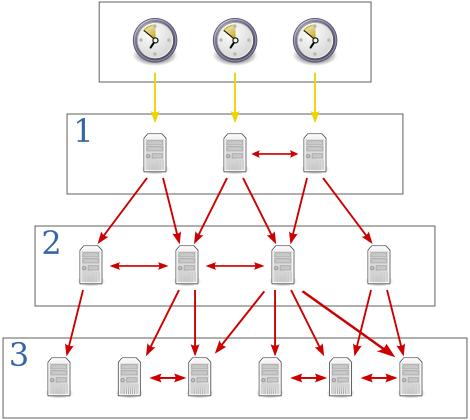
\includegraphics[width=0.7\linewidth]{Photos/HW2/levels.png}
    \caption{فلش‌های زرد نشان‌دهنده‌ی ارتباط مستقیم و فلش‌های زرد نشان‌دهنده‌ی ارتباط از طریق شبکه است.}
    \label{fig:my_label}
\end{figure}
\begin{figure}[H]
    \centering
    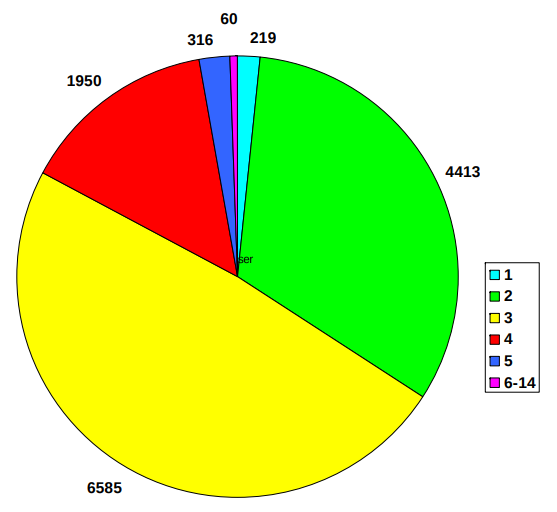
\includegraphics[width=0.85\linewidth]{Photos/HW2/stratum.png}
    \caption{مطالعه‌ی آماری سرورها، دسته‌بندی شده بر اساس
    \lr{Stratum}
    های مختلف در سال ۱۹۹۷ میلادی}
    \label{fig:my_label}
\end{figure}
در شکل 1 نمایی از سطوح ارتباطی بین
\lr{Stratum}
ها و هماهنگی آن‌ها با ساعت جهانی و در شکل 2 فراوانی هریک از آن‌ها دیده می‌شود.\\
پروتکل زمان شبکه از متد
\lr{offset delay estimation}
استفاده می‌کند.\\
در عمل یک گره منبع نمی‌تواند به طور دقیق زمان محلی را در گره هدف تخمین بزند، زیرا تاخیر و نوع پیام‌ها در شبکه متفاوت است.
\lr{NTP}
با روشی بسیار رایج تست‌های مختلف انجام داده و حداقل تاخیر را انتخاب می‌کند.\\
\begin{figure}[H]
    \centering
    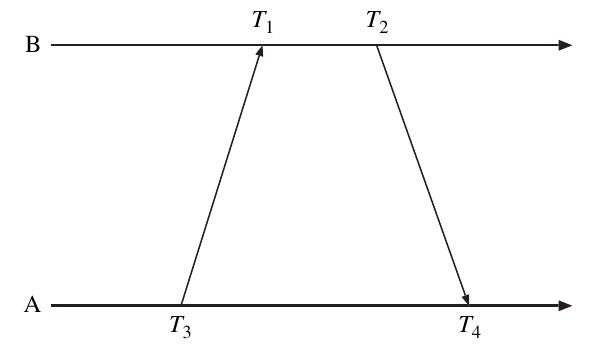
\includegraphics[width=0.99\linewidth]{Photos/HW2/delay.png}
    \caption{متد
    \lr{offset delay estimation}}
    \label{fig:my_label}
\end{figure}
شکل 3 نشان می‌دهد که چگونه 
\lr{timestamp}
ها شماره‌گذاری شده و بین زوج
\lr{A}
و
\lr{B}
مبادله شدند.\\
فرض کنیم ساعت‌های
\lr{A}
و
\lr{B}
پایدار بوده و سرعت‌های آن‌ها یکسان باشد. همچنین در نظر بگیریم:
$$a = T_1 - T_3$$
$$b = T_2 - T_4$$
اگر تفاوت تاخیر شبکه برای
\lr{A}
به
\lr{B}
با
\lr{B}
به
\lr{A}
(که به آن
\lr{differential delay}
می‌گویند)
ناچیز باشد، 
\lr{clock offset}
برابر با 
$\theta$
باشد و تاخیر رفت و برگشت از
\lr{B}
نسبت به
\lr{A}
در زمان
$T_4$
برابر
$\delta$
باشد، روابط زیر به تقریب برقرار هستند:
$$\theta = \dfrac{a + b}{2}, \delta = a - b$$
هر پیام شامل
\lr{timestamp}
های 
$T_1, T_2, T_3$
است در حالی که 
$T_4$
در زمان ورود تعیین می‌شود.\\
هر کلاینت می‌تواند به چندین تایم سرور
\lr{NTP}
همزمان متصل شده و دقیق‌ترین زمان را بدست آورد؛ علی‌الخصوص اگر نیاز به دقت بالایی باشد این مورد کاربرد بیشتری دارد.\\
ارتباط با سرورهای
\lr{NTP}
از طریق پورت
$\text{UDP}/123$
انجام می‌شود و هر زمان که درخواست رخ دهد، دقیق‌ترین ساعت مربوط به همان
\lr{Time Zone}
را به آن ارسال می‌کند.\\
عواملی چون نزدیکی سرورها نیز در دقت زمان اعلامی تأثیرگذار هستند که
\lr{NTP}
با مدیریت این موضوع می‌تواند از نزدیک‌ترین سرور به کلاینت، در خواست ساعت کند تا این درصد خطا به علت فاصله مکانی را به حداقل برساند.\\
یکی از تایم سرورهای ایران
\url{time.day.ir}
است که می‌توان کلاک دستگاه‌ها را
\lr{config}
کرده و با آن سنکرون کرد.
\rule{\linewidth}{1pt}

\section{}
\subsection{}
$$(Vt_1[1], Vt_2[2], \dots, Vt_n[n]) $$
$$= \max(Vt_1, Vt_2, \dots, Vt_n)$$
در واقع هر پروسه‌ای زمان محلی یا
\lr{Locat Time}
خود را بهتر و دقیق‌تر از بقیه‌ی پروسه‌ها می‌داند، چرا که بقیه از طریق انتقال اطلاعات آپدیت خواهند شد.\\
درایه‌ی مربوط به پروسه‌ی 
\lr{i}
در وکتور مورد نظر، فقط توسط خودش زیاد می‌شود و بقیه‌ی پروسه‌ها فقط وضعیت این درایه‌ی خاص را با دریافت پیام آپدیت می‌کنند. یعنی بزرگترین مقدار برای این درایه از وکتور، حتما در مقادیر خود آن پروسه دیده می‌شود. در نتیجه از کنار هم قرار دادن این مقادیر به ازای هر
\lr{i}
از این 
\lr{n}
پروسه، در واقع ماکزیمم مقادیر را بدست آورده‌ایم.

\subsection{}
$$e_i \rightarrow e_j \Leftrightarrow VT_{e_i}[i] < VT_{e_j}[i]$$
برای اثبات بخش اول (از چپ به راست عبارت شرطی) استدلالی مشابه سوال بند قبل خواهیم داشت. یعنی یا
\lr{event}
داخلی و یا خارجی رخ داده است و بالاخره مسیری وجود داشته که 
$e_i$
از آن طریق به
$e_j$
رسیده و اندیس
$i$
را در وکتور آپدیت کرده است. اگر این اتفاق نمی‌افتاد حتما این مقدار در وکتور خودش بزرگتر می‌بود و در نتیجه رابطه‌ی علی که به صورت فرض در نظر گرفته بودیم نقض می‌شد.\\
همچنین برای نشان دادن درستی این عبارت دوشرطی، باید بخش دوم (از راست به چپ عبارت شرطی) را نیز نشان دهیم. یعنی اگر جایی این نابرابری وجود داشت نتیجه بگیریم رابطه علی برقرار بوده است. بالاخره نقطه‌ای وجود داشته که
$i$
قبل از
$j$
رخ داده و اندیس مدنظر در وکتور آن را آپدیت کرده است. پس اگر روابط علی را به شکل یک گراف پشت این رخداد رسم کنیم، قطعا از نقطه‌ای به ادامه‌ی آن متصل شده است که یعنی رابطه‌ی علی برقرار است.\\
در نتیجه‌ی این دو بخش می‌توان نتیجه گرفت عبارت دوشرطی مذکور برقرار است.


\end{multicols}
\end{document}
